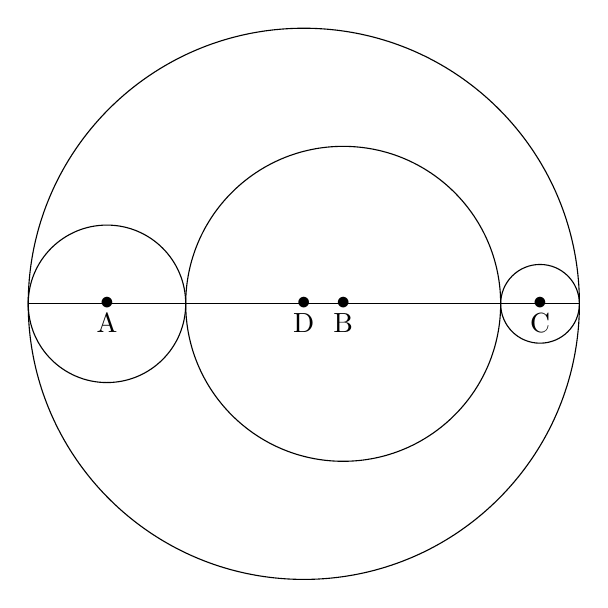
\begin{tikzpicture}
\draw (0.5,0)circle(2)node[anchor=north]{B};
\draw(-2.5,0)circle(1)node[anchor=north]{A};
\draw(3,0)circle(0.5)node[anchor=north]{C};
\draw(-2.5,0)node{$\bullet$}++(3,0)node{$\bullet$}++(2.5,0)node{$\bullet$};
\draw(0,0)circle(3.5);
\draw(-3.5,0)--(3.5,0);
\draw(0,0)node{$\bullet$}node[anchor=north]{D};
\end{tikzpicture}
Circle A has a radius of $2$. Circle B has a radius of $8$. Circle C has a radius of $4$.  All the circles are tangent to each other as shown.  What is the radius of circle D?


\ifsat
	\begin{enumerate}[label=\Alph*)]
		\item  $7$
		\item  $8$
		\item  $14$%
		\item  $16$
	\end{enumerate}
\else
\fi

\ifacteven
	\begin{enumerate}[label=\textbf{\Alph*.},itemsep=\fill,align=left]
		\setcounter{enumii}{5}
		\item  $7$
		\item  $8$
		\item  $14$%
		\addtocounter{enumii}{1}
		\item  $16$
		\item  $28$
 
	\end{enumerate}
\else
\fi

\ifactodd
	\begin{enumerate}[label=\textbf{\Alph*.},itemsep=\fill,align=left]
		\item  $7$
		\item  $8$
		\item  $14$%
		\item  $16$
		\item  $28$
 
	\end{enumerate}
\else
\fi

\ifgridin
  $14$%
		
\else
\fi

